%!TEX root = ../main.tex

\begin{newpage}
	
	\section{Grundlagen}
	\label{sec:Grundlagen}

	\subsection{Das GTFS Datenformat}
	\label{ssec:das_gtfs_datenformat}
    % zur ... entwickelt wurde.
		Das GTFS (General Transit Feed Specification) ist eine Datenstandardisierung die von Google im Jahr 2006 entwickelt wurde. Dies ermöglichte es Transit Organisationen ihre Daten für dritte zur Verfügung zu stellen und auszutauschen. Ein GTFS Feed besteht dabei aus mindestens 6 und maximal 13 \texttt{csv-Dateien}, die im \texttt{.txt} Format vorliegen müssen. Die Struktur eines Feeds lässt sich in Worten wie folgt beschreiben:

    \begin{quote}
      \textit{Ein GTFS Feed besteht aus einer oder mehreren Routen. Jede Route (\texttt{routes.txt}) hat einen oder mehrere Trips (\texttt{trips.txt}). Jeder Trip besucht eine Abfolge von Stops (\texttt{stops.txt}) zu einer bestimmten Zeit (\texttt{stop\_times.txt}). Trips und Stop-Zeit beinhalten nur die Tageszeit Informationen. Der Kalender (calendar.txt und \texttt{calendar\_dates.txt}) bestimmt dann, an welchen Tagen ein bestimmter Trip stattfindet.} \parencite[S. 8]{zervaas}
    \end{quote}


    % Einheitliche Form (müsste oder muss). Deutschland immer noch keine breite Standardisierung (gegenüber USA). Deshalb die hier beschriebenen (folgenden) Probleme. 

		Vor der Einführung gab es keinerlei standardisiertes Format für die Fahrpläne des Öffentlichen Nahverkehrs in den USA. Leider ist in Deutschland die Standardisierung Vor allem für digitale Produkte, wie zum Beispiel Trip-Planer, die viele verschiedene Verkehrsverbundsnetze in ihren Service integrieren müssen, ist ein standardisiertes Datenformat unbedingt notwendig. 
		Ohne einen Standard müsste jede App die Entwickelt wird, auf das Datenformat der jeweiligen Verkehrsunternehmen angepasst werden. Das wiederum bedeutet, dass je nach Implementierung innerhalb dieser Unternehmen, die Datenformate gänzlich voneinander abweichen können. Für jeden dieser Anbieter müsste folglich eine ganz eigene Datenverarbeitungslogik geschrieben werden.
    Darüber hinaus könnte natürlich jedes Verkehrsunternehmen jederzeit sein eigenes Datenformat ändern, was zur Folge hat, dass ein App-Entwickler diese Änderungen auch in sein Produkt übernehmen muss. Bei einer Integration von Daten, aus beliebig vielen unterschiedlichen Verkehrsunternehmen (Beispiel: Trip-Planer für ganz Deutschland), könnten sich laufend Änderungen ergeben die integriert werden müssen, oder das eigene Produkt würde nicht mehr zuverlässig funktionieren. Dies übersteigt die Wartbarkeit und Robustheit einer App, denn sie würde möglicherweise immer dann nicht mehr funktionieren, wenn ein Dritter entscheidet sein eigenes Datenformat zu ändern.\\

    Allerdings ergeben sich trotz der Standardisierung durch GTFS immer noch diverse Freiräume in der Umsetzung des Formats. Wie anfangs erwähnt wurde, beträgt die Anzahl der Dateien die für ein gültiges GTFS Feed benötigt werden nur Sechs. Es sind allerdings bis zu 13 Dateien möglich. Dies zeigt wie viele unterschiedliche Informationen ein GTFS Feed bereitstellen kann, aber nicht muss. 
    Auch innerhalb der Dateien gibt es Felder die vorhanden sein "`müssen"' oder nur "`dürfen"'. Beispielsweise muss das Feld \texttt{route\_short\_name} in \texttt{routes.txt} vorhanden sein, aber \texttt{route\_desc} (Route Description) nicht. Der Interpretationsspielraum lässt sich aber noch weiter veranschaulichen, wenn wir uns Tabelle ~\ref{table:gtfs_differences} ansehen. In dieser Tabelle sind Zwei Einträge aus unterschiedlichen GTFS Feeds aufgelistet.
    Wir sehen, dass die Spalte \texttt{route\_id} bei Stuttgart-VVS als Zahlenwert angegeben wird, wohingegen Boston-MBTA einen Text verwendet.

    \begin{longtable}{|>{\raggedright \arraybackslash}p{3.0cm}|>{\raggedright \arraybackslash}p{1.5cm}|>{\raggedright \arraybackslash}p{3.5cm}|>{\raggedright \arraybackslash}p{6.0cm}|}
    \caption{Unterschiede innerhalb GTFS} 
    \label{table:gtfs_differences}\\
      \hline
       & route\_id & route\_short\_name & route\_long\_name\\
      \hline
      Stuttgart-VVS & 379 & U1 & Fellbach - Hauptbahnhof - Vaihingen\\
      \hline
      Boston-MBTA & Blue Line & Blue & Rapid Transit\\
      \hline
    \end{longtable}

    % Die fehlende/nicht gegebene Übereinstimmung beim Gebrauch der Variablen führt als zu Problemen bei der ...

    Allerdings ist die "`Blue Line"' die Beschreibung einer U-Bahnlinie\parencite{wiki_blue_line}. Wir sehen also, dass Stuttgart-VVS die \texttt{route\_id} zur eindeutigen Identifizierung mittels Zahlenwert (ID) verwendet, während Boston-MBTA dieses Feld nutzt, um neben der Identifizierung gleichzeitig auch die Beschreibung der Linie zu liefern. Angenommen wir hätten ein Element in einer Benutzeroberfläche, die dieses Feld auslesen und anzeigen würde, dann sehen wir in Abbildung ~\ref{fig:gtfs_differences} links eine korrekte Information bei Verwendung des Boston-MBTA Feeds und rechts eine numerische ID des Stuttgart-VVS Feeds die keinerlei Bedeutung hat und an dieser Stelle falsch ist.

    \begin{figure}[htbp]
      \begin{center}
        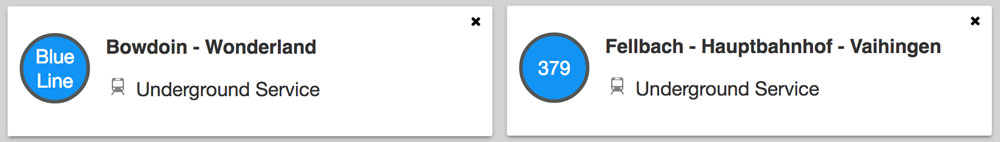
\includegraphics[width=\textwidth]{gtfs_differences.jpg}
        \caption{Description}
        \label{fig:gtfs_differences}
      \end{center}
    \end{figure}
    
    
    
		Unter anderem aus diesem Grund erfolge die Adaption an das GTFS Format erfolgte schnell und so ist heute der größte teil der Fahrpläne als GTFS Feed frei verfügbar auf Plattformen wie: \url{http://transitfeeds.com} zu finden. 

		Da das GTFS-Format das grundlegende Datenformat für diese Arbeit ist, sollen nachfolgend kurz die wichtigsten beschrieben werden.

		\begin{itemize}
			\item \texttt{agency.txt}: Beinhaltet Informationen über die Verkehrsunternehmen, welche das Feed und die Daten bereitstellen.

			\item \texttt{routes.txt}: Eine Route ist eine Gruppierung von Trips. Die verschiedenen Eigenschaften einer Route werden in dieser Tabelle gespeichert.

			\item \texttt{trips.txt}: Ein Trip gehört zu einer Route. Eine Route kann dabei beliebig viele Trips haben. Welche Trips aktiv sind wird durch den Kalender festgelegt.

			\item \texttt{calendar.txt}: Bestimmt, an welchen Tagen ein Trip aktiv ist.

			\item \texttt{stop\_times.txt}: Diese Tabelle beschreibt welche Stationen nacheinander angefahren werden. Für jede Station beinhaltet sie die Ankunfts- und Abfahrtszeiten.

			\item \texttt{stops.txt}: Stellt nähere Informationen für jede Station zur Verfügung wie zum Beispiel den Stationsnamen und deren Position.

			\item \texttt{shapes.txt}: Jeder Trip kann eine dazugehörigen Polyline\footnote{Linienverlauf} haben. Eine Polyline ist dabei nichts anderes als eine Abfolge von Punkten, die, wenn man sie verbindet, eine Linie ergeben. Um einen Routenverlauf auf eine Karte zu zeichnen, wird diese Tabelle folglich unbedingt benötigt. 
		\end{itemize}

	\section{Existierende Projekte}
	\label{sec:existierende_projekte}

\end{newpage}
% section grundlagen